Using the described algorithm, four models were computed. Two using the linear classifier and two using the random forest. As ten videos have training data the dataset was split into training and testing sets. One linear and forest model was trained with the videos 1 to 4 (named A) and one with the videos 5 to 8 (named B). Because of memory restrictions in the working machine the sets could not be larger. With these models the training videos were processed and the predictions saved.
\subsection{Labeling performance} % (fold)
\label{sub:labeling_precision}
To get some performance measurement all four models were used on the complementary trainings data. Therefor the original hand-labeled boxes were put into the models and the predicted labels were compared with the original label. Both methods only predict classes and no floating point score so one data-wide precision and recall value was calculated. The precision is the fraction of the as road predicted instances that are actually road. The recall is the fraction of all road instances that were predicted. Additionally we look at the F-measure.
As seen in \autoref{tab:measure_table} all ratings are above 0.98 and therefore show that all four models reached a high accuracy in predicting  the complementing testing data. The random forest trained on videos 5 to 8 performed slightly better then the other three. Nevertheless is this performance not inevitably transferred into the visually seen performance to predict the actual roadway shape. Without a more, near pixel accurate labeling of the roadways the actual desired classification performance can not be measured.
\begin{table}
	\footnotesize
	\centering
	\begin{tabular}{p{1.7cm}cccc}
	& linear A & forest A & linear B & forest B \\
	\toprule \\
	Precision & 0.9865 & 0.9899 & 0.9854 & 0.9893 \\
	Recall & 0.9938 & 0.9899 & 0.9942 & 0.9923 \\
	F-Measure & 0.9901 & 0.9899 & 0.9898 & 0.9908\\
	\toprule
	\end{tabular}
	\caption{Performance measurements for the models}
	\label{tab:measure_table}
\end{table}
% subsection labeling_precision (end)i

\subsection{Time performance} % (fold)
\label{sub:time_costs}
The application of such algorithms in the real world strongly depends on good time performance. A car without real time information processing and decision system is mostly pointless. Also because of my own technical limitations there was a strong focus on processing speed. Stopping the time for reading the frame, making the prediction and applying the Morphology but without possible saving operations the ranges of time periods is visualized for the four models and \texttt{seq0000} in \autoref{fig:time_plot}.
\begin{figure}
	\centering
	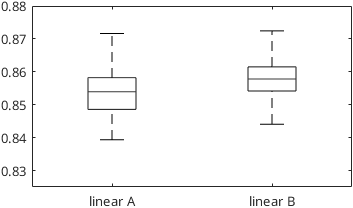
\includegraphics[width=0.4\columnwidth,keepaspectratio]{linear_time_measures_bw}
	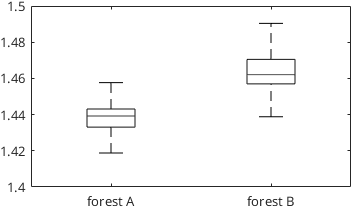
\includegraphics[width=0.4\columnwidth,keepaspectratio]{forest_time_measures_bw}
	\caption{Ranges of processing times in seconds}
	\label{fig:time_plot}
\end{figure}
\texttt{LibLinear} performed clearly faster in both trainings set cases than the random forests. This depends mostly only on the actual prediction time the libraries take. All models process a frame in under 1.5sec. With linear classification the prediction takes way under a second which was aimed at. Taken the nearly same labeling performance into account the speed seems a huge drawback of using a random forest.\\
Most task were able to be calculated in parallel on the multi-core CPU but as I have seen the factor of around $\frac{1}{4}$ is not as helpful as an focus on a fast implementation.
% subsection time_costs (end)